%% -*- Lecture -*-

\documentclass[11pt,aspectratio=169]{beamer}

\usepackage[oldspacing]{rcstalk}
\usetheme{rcstheme}

\subtitle{Lecture 5: Synchronization}
\topic{Concurrency}

\begin{document}

\maketitle

\section{Synchronization and memory consistency review}

\begin{slide}{Motivation}
$$ T(n) = T(1)\left(B + \frac{1}{n} (1 - B)\right) $$

\itms{
  \item Amdahl's law
  \ittms {
    \item $T(1)$: the time one core takes to complete the task
    \item $B$: the fraction of the job that must be serial
    \item $n$: the number of cores
  }
  \item Suppose $n$ were infinity!
  \item Amdahl's law places an ultimate limit on parallel speedup
  \item Problem: synchronization increases serial section size
  \gap
  \item Scalable Commutativity Rule: \emph{``Whenever interface operations 
      commute, they can be implemented in a way that scales''} 
      \href{http://web.mit.edu/amdragon/www/pubs/commutativity-sosp13.pdf}{[Clements]}
}
\end{slide}

\begin{slide}{Locking Basics}
\begin{smallccode}
    pthread_mutex_t m;

    pthread_mutex_lock(&m);
    cnt = cnt + 1; /* critical section */
    pthread_mutex_unlock(&m);
\end{smallccode}
\itms{
  \item Only one thread can hold a lock at a time
  \item Makes critical section atomic
  \item When do you need a lock?
  \ittms {
    \item Anytime two or more threads touch data and at least one writes
  }
  \item Rule: Never touch data unless you hold the right lock
}
\end{slide}

\begin{slide}{Fine-grained Locking}
\begin{smallccode}
    struct list_head *hash_tbl[1024];

    /* Coarse-grained Locking */
    mutex_t m;
    mutex_lock(&m);
    struct list_head *pos = hash_tbl[hash(key)];
    /* walk list and find entry */
    mutex_unlock(&m);

    /* Fine-grained Locking */
    mutex_t bucket[1024];
    int index = hash(key);
    mutex_lock(&bucket[index]);
    struct list_head *pos = hash_tbl[index];
    /* walk list and find entry */
    mutex_unlock(&bucket[index]);
\end{smallccode}
\itms{
  \item Which of these is better?
}
\end{slide}
 
% \begin{slide}{Readers-Writers Problem}
% \itms{
%   \item Recall a \texttt{mutex} allows in only one thread
%   \item But a data race occurs only if
%   \begin{itemize}
%     \item multiple threads access the same data, \alert{and}
%     \item at least one of the accesses is a write
%   \end{itemize}
%   \item How to allow multiple readers \emph{or} one single writer?
%   \ittms{
%     \item Need lock that can be \emph{shared} amongst concurrent readers
%   }
%   %% \item Multiple threads may access data
%   %% \ittms{
%   %%   \item \emph{Readers} -- will only observe, not modify data
%   %%   \item \emph{Writers} -- will change the data
%   %% }
%   \item Can implement using other primitives (next slide)
%   \ittms{
%     \item Keep integer \texttt{i} -- \# or readers or -1 if held by writer
%     \item Protect \texttt{i} with mutex
%     \item Sleep on condition variable when can't get lock
%   }
% }
% \end{slide}
% 
% % \begin{slide}{Implementing shared locks}
% % \begin{smallccode}
% % struct sharedlk {
% %   int i;     /* # shared lockers, or -1 if exclusively locked */
% %   mutex_t m;
% %   cond_t c;
% % };
% % 
% % void AcquireExclusive (sharedlk *sl) {
% %   lock (sl->m);
% %   while (sl->i) { wait (sl->m, sl->c); }
% %   sl->i = -1;
% %   unlock (sl->m);
% % }
% % 
% % void AcquireShared (sharedlk *sl) {
% %   lock (sl->m);
% %   while (sl->i < 0) { wait (sl->m, sl->c); }
% %   sl->i++;
% %   unlock (sl->m);
% % }
% % \end{smallccode}
% % \end{slide}
% 
% % \begin{slide}{shared locks (continued)}
% % \begin{smallccode}
% % void ReleaseShared (sharedlk *sl) {
% %   lock (sl->m);
% %   if (!--sl->i) signal (sl->c);
% %   unlock (sl->m);
% % }
% % 
% % void ReleaseExclusive (sharedlk *sl) {
% %   lock (sl->m);
% %   sl->i = 0;
% %   broadcast (sl->c);
% %   unlock (sl->m);
% % }
% % \end{smallccode}
% % \itms{
% %   \item Note:  Must deal with starvation
% % }
% % \end{slide}
% 
% \begin{slide}{Review: Test-and-set spinlock}
% \begin{smallccode}
%     struct var {
%       int lock;
%       int val;
%     };
% 
%     void atomic_inc (var *v) {
%       while (test_and_set (&v->lock))   
%         ;
%       v->val++;
%       v->lock = 0;
%     }
% 
%     void atomic_dec (var *v) {
%       while (test_and_set (&v->lock))   
%         ;
%       v->val--;
%       v->lock = 0;
%     }
% \end{smallccode}
% \begin{itemize}
%   \item Is this code correct without sequential consistency?
% \end{itemize}
% \end{slide}
% 
\begin{frame}[fragile]
\frametitle{Memory reordering danger}
\itms{
  \item Suppose no sequential consistency \& don't compensate
  \item Hardware could violate program order
}
\centerline{\small\vbox{\offinterlineskip
\halign{\strut\hfil #&\texttt{#}\hfil&\qquad\texttt{#}\hfil\cr
\multispan2{\hfil \color{comment}\normalsize Program order on CPU \#1\hfil}
 &\omit{\qquad\hfil\color{comment}\normalsize View on CPU \#2}\hfil\cr
\multispan3{\vrule width0pt height 2pt}\cr
\multispan2{\hrulefill}&\omit\qquad\hrulefill\cr
\multispan3{\vrule width0pt height 2pt}\cr
read/write: & v->lock = 1;              & v->lock = 1;\cr
      read: & register = v->val;\cr
\Red{write:} & \tikz[remember picture,baseline=(progorder.base)]%
               {\node[red,inner sep=0] (progorder) {v->val = register + 1;};}\cr
     write: & v->lock = 0;              & v->lock = 0;\cr
&&\color{comment}/* danger */\cr
&&\tikz[remember picture,baseline=(otherorder.base)]%
               {\node[red,inner sep=0] (otherorder) {v->val = register + 1;};}\cr
}}}
\begin{tikzpicture}[remember picture,overlay]
\draw[->,thick] (progorder.east) to (otherorder.north west);
\end{tikzpicture}
\itms{
  \item If \texttt{atomic\_inc} called at
    {\color{comment}\texttt{/* danger */}}, bad \texttt{val} ensues!
}
\end{frame}
 
\begin{frame}[fragile]
\frametitle{Ordering requirements}
\begin{ccode}
    void atomic_inc (var *v) {
      while (test_and_set (&v->lock))
        ;
      v->val++;
      `\alt<-2>{{\color{comment}/* danger */}}{{\color{red}asm volatile ("sfence" ::: "memory");}}'
      v->lock = 0;
    }
\end{ccode}
\begin{itemize}
  \item Must ensure all CPUs see the following:
  \begin{enumerate}
    \item \texttt{v->lock} was set \emph{before} \texttt{v->val}
      was read and written
    \item \texttt{v->lock} was cleared \emph{after} \texttt{v->val}
      was written
  \end{enumerate}
  \item How does \#1 get assured on x86?
  \begin{itemize}
    \item Recall \verb+test_and_set+ uses \verb+xchgl %eax,(%edx)+
\onslide<2->{
    \item \texttt{xchgl} instruction always ``locked,'' ensuring
      barrier
}
  \end{itemize}
  \item How to ensure \#2 on x86?
  \begin{itemize}
      \onslide<3->{\item Might need fence instruction after, e.g.,
          non-temporal stores}
  \end{itemize}
\end{itemize}
\end{frame}

\begin{slide}{MIPS Spinlocks}
\vspace{-1em}
\itms{
  \item \texttt{LL rt, offset(rb)} -- Load Linked
  \ittms{
    \item \code{rt} $\leftarrow$ \code{memory[rb+offset]}
  }
  \item \texttt{SC rt, offset(base)} -- Store conditional (sets rt 0 if not 
      atomic)
  \ittms{
    \item if atomic w.r.t. prior LL \code{memory[rb+offset]} $\leftarrow$ 
	\code{rt, rt} $\leftarrow$ \code{1}
    \item else \code{rt} $\leftarrow$ \code{0}
  }
}
\begin{mipsasm}
# spinlock_data_t spinlock_data_testandset(spinlock_data_t *sd)
    ll      v0, 0(a0)           # v0 = *sd (Load Linked)
    addi    t1, zero, 1         # t1 = 1
    sc      t1, 0(a0)           # *sd = t1 (Store Conditional)
    bne     t1, zero, 1f        # if SC not failed
    nop                         # branch delay slot
    addi    v0, zero, 1         # return 1 on failure
1:  j       ra                  # return to caller
    nop                         # branch delay slot
\end{mipsasm}
\itms{
  \item MIPS I (SYS/161) is sequentially consistent $\rightarrow$ no barriers 
      needed
  \item Later MIPS processors need \code{SYNC} memory barrier
}
\end{slide}

\begin{slide}{OS/161 Spinlock Acquire}
\begin{smallccode}
void spinlock_acquire(struct spinlock *lk)
{
  struct cpu *mycpu;
  
  splraise(IPL_NONE, IPL_HIGH);
  
  /* this must work before curcpu initialization */
  if (CURCPU_EXISTS()) {
    mycpu = curcpu->c_self;
    if (lk->lk_holder == mycpu) {
      panic("Deadlock on spinlock %p\n", lk);
    }
  } else {
    mycpu = NULL;
  }
  ...
}
\end{smallccode}
\end{slide}

\begin{slide}{OS/161 Spinlock Acquire Con't}
\begin{smallccode}
void spinlock_acquire(struct spinlock *lk)
{
  ...
  while (1) {
    /*
     * First check if the lock is busy to reduce
     * coherence traffic (more on this later).
     */
    if (spinlock_data_get(&lk->lk_lock) != 0) {
      continue;
    }
    /* Attempt to acquire the lock */
    if (spinlock_data_testandset(&lk->lk_lock) != 0) {
      continue;
    }
    break;
  }
  lk->lk_holder = mycpu;
}
\end{smallccode}
\end{slide}

\

% \begin{slide}{Correct spinlock on alpha}
% \itms{
%   \item \texttt{ldl\_l} -- load locked \\
%         \texttt{stl\_c} -- store conditional (sets reg to 0 if not atomic
%         w.\ \texttt{ldl\_l})
% }
% \begin{alphaasm}
%    _test_and_set:
% 	ldq_l   $v0, 0($a0)           # v0 = *lockp (LOCKED)
% 	bne     $v0, 1f               # if (v0) return
% 	addq    $zero, 1, $v0         # v0 = 1
% 	stq_c   $v0, 0($a0)           # *lockp = v0 (CONDITIONAL)
% 	beq     $v0, _test_and_set    # if (failed) try again
%         `{\color{red}mb}'
% 	addq    $zero, $zero, $v0     # return 0
%    1:   ret     $zero, ($ra), 1
% \end{alphaasm}
% \itms{
%   \item Note: Alpha memory consistency much weaker than x86
%   \item Must insert \emph{memory barrier} instruction,
%     \Red{\texttt{mb}} (like \texttt{mfence})
%   \begin{itemize}
%     \item All processors will see that everything before \texttt{mb}
%       in program order happened before everything after \texttt{mb} in
%       program order
%   \end{itemize}
% }
% \end{slide}
% 
% \begin{slide}{Memory barriers/fences}
% \itms{
%   \item Must use memory barriers (a.k.a.\ fences) to preserve program
%     order of memory accesses with respect to locks
%   %% \item \texttt{mb} in \texttt{test\_and\_set} preserves program order
%   %% \ittms{
%   %%   \item All ops before \texttt{mb} in program order appear before on
%   %% \emph{all CPUs}
%   %%   \item All ops after \texttt{mb} in program order appear after on
%   %% \emph{all CPUs}
%   %% }
%   \item Many examples in this lecture assume S.C.
%   \ittms{
%     \item Useful on non-S.C. hardware, but must add barriers
%   }
%   \item Dealing with memory consistency important
%   \ittms{
%     \item See
%       \href{http://www.kernel.org/doc/Documentation/memory-barriers.txt}{[Howells]}
%       for how Linux deals with memory consistency
%     \item
%       \href{http://en.cppreference.com/w/cpp/atomic/memory_order}{C++}
%       now exposes support for different memory orderings
%   }
%   \item Fortunately, consistency need not overly complicate code
%   \ittms{
%     \item If you do locking right, only need to add a few barriers
%     \item Code will be easily portable to new CPUs
%   }
% }
% \end{slide}

\section{C11 Atomics}

\begin{slide}{Atomics and Portability}
\itms{
  \item Lots of variation in atomic instructions, consistency models, compiler behavior
  \item Results in complex code when writing portable kernels and applications
  \item Still a big problem today: Your laptop is x86, your cell phone is ARM
  \ittms{
    \item x86: Total Store Order Consistency Model, CISC
    \item arm: Relaxed Consistency Model, RISC
  }
  \item Fortunately, the new C11 standard has builtin support for atomics
  \ittms{
    \item Enable in GCC with the \texttt{-std=c11} flag
  }
  \item Also available in C++11, but not discussed today...
}
\end{slide}

\begin{slide}{C11 Atomics: Basics}
\ittms{
  \item Portable support for synchronization
  \item New atomic type: e.g., \texttt{\_Atomic(int) foo}
  \ittms {
    \item All standard ops (e.g., $+$, $-$, $/$, $*$) become sequentially 
	consistent
    \item Plus new intrinsics available (cmpxchg, atomic increment, etc.)
  }
  \item \texttt{atomic\_flag} is a special type
  \ittms {
    \item Atomic boolean value without support for loads and stores
    \item Must be implemented lock-free
    \item All other types might require locks, depending on the size and architecture
  }
  \item Fences also available to replace hand-coded memory barrier assembly
}
\end{slide}

\begin{slide}{Memory Ordering}
\ittms{
  \item several choices available
  \begin{enumerate}
    \item \texttt{memory\_order\_relaxed}: no memory ordering
    \item \texttt{memory\_order\_consume}
    \item \texttt{memory\_order\_acquire}
    \item \texttt{memory\_order\_release}
    \item \texttt{memory\_order\_acq\_rel}
    \item \texttt{memory\_order\_seq\_cst}: full sequential consistency
  \end{enumerate}
  \item What happens if the chosen model is mistakenly too weak? Too Strong?
  \item Suppose thread 1 \textbf{releases} and thread 2 \textbf{acquires}
  \ittms {
    \item Thread 1's preceding \textbf{writes} can't move past the \textbf{release} store
    \item Thread 2's subsequent \textbf{reads} can't move before the \textbf{acquire} load
    \item Warning: other threads might see a completely different order
  }
}

\end{slide}

\begin{slide}{Example 1: Atomic Counters}
\begin{smallccode}
    _Atomic(int) packet_count;

    void recv_packet(...) {
        ...
        atomic_fetch_add_explicit(&packet_count, 1,
            memory_order_relaxed);
        ...
    }
\end{smallccode}
\end{slide}

\begin{slide}{Example 2: Producer, Consumer}
\begin{smallccode}
    struct message msg_buf;
    _Atomic(_Bool) msg_ready;

    void send(struct message *m) {
        msg_buf = *m;
        atomic_thread_fence(memory_order_release);
        atomic_store_explicit(&msg_ready, 1,
            memory_order_relaxed);
    }

    struct message *recv(void) {
        _Bool ready = atomic_load_explicit(&msg_ready,
            memory_order_relaxed);
        if (!ready)
            return NULL;
        atomic_thread_fence(memory_order_acquire);
        return &msg_buf;
    }
\end{smallccode}
\end{slide}

\begin{slide}{Example 3: A Spinlock}
\itms{
    \item Spinlocks are similar to Mutexes
    \item Kernel's use these for small critical regions
    \ittms{
	\item Busy wait for others to release the lock
	\item No sleeping and yielding to other Threads
    }
    \gap
}
\begin{smallccode}
    void spin_lock(atomic_flag *lock) {
        while(atomic_flag_test_and_set_explicit(lock,
            memory_order_acquire)) {}
    }

    void spin_unlock(atomic_flag *lock) {
        atomic_flag_clear_explicit(lock, memory_order_release);
    }
\end{smallccode}

\end{slide}

\section{Cache coherence -- the hardware view}

\begin{slide}{Overview}
\itms{
  \item Coherence
  \ittms{
    \item concerns accesses to a single memory location
    \item makes sure stale copies do not cause problems
  }
  \item Consistency
  \ittms{
    \item concerns apparent ordering between multiple locations
  }
}
\end{slide}

\begin{slide}{Multicore Caches}
\vspace{-1em}
\itms{
  \item Performance requires caches
  \item Caches create an opportunity for cores to disagree about memory
  \item Bus-based approaches
  \ittms{
    \item ``Snoopy'' protocols, each CPU listens to memory bus
    \item Use write through and invalidate when you see a write
      bits
    \item Bus-based schemes limit scalability
  }
  \gap
  \item Modern CPUs use networks (e.g., hypertransport, UPI)
  % and message passing
  \item Cache is divided into chuncks of bytes called {\em cache lines}
  \ittms{
    \item 64-bytes is a typical size
  }
}
\end{slide}

\begin{slide}{3-state Coherence Protocol (MSI)}
\itms{
  \item Each cache line is one of three states:
  \gap
  \item Modified (sometimes called Exclusive)
  \ittms{
    \item One cache has a valid copy
    \item That copy is stale (needs to be written back to memory)
    \item Must invalidate all copies before entering this state
  }
  \item Shared
  \ittms{
    \item One or more caches (and memory) have a valid copy
  }
  \item Invalid
  \ittms{
    \item Doesn't contain any data
  }
  \item Transitions can take 100--2000 cycles
}
\end{slide}

\begin{slide}{Core and Bus Actions}
\itms{
  \item Core has three actions:
  \item Read (load)
  \ittms{
    \item Read without intent to modify, data can come from memory or another 
	cache
    \item Cacheline enters shared state
  }
  \item Write (store)
  \ittms{
    \item Read with intent to modify, must invalidate all other cache copies
    \item Cacheline in shared (some protocols have an exclusive state)
  }
  \item Evict
  \ittms{
    \item Writeback contents to memory if modified
    \item Discard if in shared state
  }
}
\end{slide}

\begin{slide}{Implications for Multithreaded Design}
\vspace{-1em}
\itms{
  \item Lesson \#1: Avoid false sharing
  \ittms{
    \item Processor shares data in cache line chunks
    \item Avoid placing data used by different threads in the same cache line
  }
  \gap
  \item Lesson \#2: Align structures to cache lines
  \ittms{
    \item Place related data you need to access together
    \item Alignment in C11/C++11: \code{alignas(64) struct foo f;}
  }
  \gap
  \item Lesson \#3: Pad data structures
  \ittms{
    \item Arrays of structures lead to false sharing
    \item Add unused fields to ensure alignment
  }
  \gap
  \item Lesson \#4: Avoid contending on cache lines
  \ittms{
    \item Reduce costly cache coherence traffic
    \item Advanced algorithms spin on a cache line local to a core (e.g., MCS 
	Locks)
  }
}
\end{slide}

% \begin{slide}{cc-NUMA}
% \itms{
% \item Previous slide had \emph{dance hall} architectures
% \ittms{
%   \item Any CPU can ``dance with'' any memory equally
% }
% \item An alternative: Non-Uniform Memory Access
% \ittms{
%   \item Each CPU has fast access to some ``close'' memory
%   \item Slower to access memory that is farther away
%   \item Use a directory to keep track of who is caching what
% }
% \item Originally for machines with many CPUs
% \ittms{
%   \item But AMD Opterons integrated mem.\ controller, essentially NUMA
%   \item Now intel CPUs are like this, too
% }
% \item cc-NUMA = cache-coherent NUMA
% \ittms{
%   \item Can also have non-cache-coherent NUMA, though uncommon
%   \item BBN Butterfly 1 has no cache at all
%   \item Cray T3D has local/global memory
% }}
% \end{slide}
% 
% \begin{slide}{Real World Coherence Costs}
% \itms{
%   \item See
%       \cref{sched/readings/david-synchronization.pdf}{[David]}
%       for a great reference, summarized here...
%   \ittms{
%     \item Intel Xeon: 3 cycle L1, 11 cycle L2, 44 cycle LLC, 355 cycle RAM
%   }
%   \item Remote core holds modified line state:
%   \ittms{
%     \item load: 109 cycles (LLC $+$ 65)
%     \item store: 115 cycles (LLC $+$ 71)
%     \item atomic CAS: 120 cycles (LLC $+$ 76)
%     \item NUMA load: 289 cycles
%     \item NUMA store: 320 cycles
%     \item NUMA atomic CAS: 324 cycles 
%   }
%   \item But only a partial picture
%   \ittms{
%     \item Could be faster because of out-of-order execution
%     \item Could be slower because of bus contention or multiple hops
%   }
% }
% \end{slide}

% \begin{slide}{Improving Spinlocks}
% \itms{
%   \item Test-and-set spinlock has several advantages
%   \ittms{
%     \item Simple to implement and understand
%     \item One memory location for arbitrarily many CPUs
%   }
%   \item But also has disadvantages
%   \ittms{
%     \item Lots of traffic over memory bus (especially when $>1$
%       spinner)
%     \item Not necessarily fair (same CPU acquires lock many times)
%     \item Even less fair on a NUMA machine
%     \item Allegedly Google had fairness problems even on Opterons
%   }
%   \item Idea 1: Avoid spinlocks altogether
%   \item Idea 2: Reduce bus traffic with better spinlocks
%   \ittms{
%     \item Design lock that spins only on local memory
%     \item Also gives better fairness
%   }
% }
% \end{slide}

% \section{Avoiding locks}
% 
% \defverbatim[colored,width=55mm]\producer{
% \begin{ccode}
% /* PRODUCER */
% for (;;) {
%   item *nextProduced
%     = produce_item ();
% 
%   mutex_lock (&mutex);
%   while (count == BUF_SIZE)
%     cond_wait (&nonfull,
%                 &mutex);
% 
%   buffer [in] = nextProduced;
%   in = (in + 1) % BUF_SIZE;
%   count++;
%   cond_signal (&nonempty);
%   mutex_unlock (&mutex);
% }    
% \end{ccode}}
% 
% \defverbatim[colored,width=55mm]\consumer{
% \begin{ccode}
% /* CONSUMER */
% for (;;) {
%   mutex_lock (&mutex);
%   while (count == 0)
%     cond_wait (&nonempty,
%                 &mutex);
% 
%   nextConsumed =  buffer[out];
%   out = (out + 1) % BUF_SIZE;
%   count--;
%   cond_signal (&nonfull);
%   mutex_unlock (&mutex);
% 
%   consume_item (nextConsumed);
% }
% \end{ccode}}
% 
% \begin{frame}
% \frametitle{Recall producer/consumer (lecture 3)}
% \begin{columns}[t]
% \column{59mm}
% \producer
% \column{60mm}
% \consumer
% \end{columns}
% \end{frame}
% 
% \begin{slide}{Eliminating locks}
% \itms{
%   \item One use of locks is to coordinate multiple updates of single
% 	  piece of state
%   \item How to remove locks here? 
%   \ittms{
%     \item Factor state so that each variable only has a single writer
%   }
%   \item Producer/consumer example revisited
%   \ittms{
%     \item Assume you have sequential consistency
%     \item Assume one producer, one consumer
%     \item \Red{Why do we need \texttt{count} variable, written by both?}  \\
%       \textsl{To detect buffer full/empty}
%     \item Have producer write \texttt{in}, consumer write \texttt{out}
%     \item Use \texttt{in}/\texttt{out} to detect buffer state
%     \item But note next example busy-waits, which is less good
%   }
% }
% \end{slide}
% 
% \begin{slide}{Lock-free producer/consumer}
% \begin{smallccode}
%      void producer (void *ignored) {
%          for (;;) {
%              item *nextProduced = produce_item ();
%              while (((in + 1) % BUF_SIZE) == out)
%                  thread_yield ();
%              buffer [in] = nextProduced;
%              release_barrier();
%              in = (in + 1) % BUF_SIZE;
%          }    
%      }
% \end{smallccode}
% \begin{smallccode}
%      void consumer (void *ignored) {
%          for (;;) {
%              while (in == out)
%                  thread_yield ();
%              nextConsumed =  buffer[out];
%              acquire_barrier();
%              out = (out + 1) % BUF_SIZE;
%              consume_item (nextConsumed);
%          }
%      }       
% \end{smallccode}
% \end{slide}
% 
% \begin{slide}{Non-blocking synchronization}
% \itms{
%   \item Design algorithm to \emph{avoid critical sections}
%   \ittms{
%     \item Any threads can make progress if other threads are preempted
%     \item Which wouldn't be the case if preempted thread held a lock
%   }
%   \item Requires atomic instructions available on many CPUs
%   \item E.g., atomic compare and swap: \texttt{CAS (mem, old, new)}
%   \ittms{
%     \item If \texttt{*mem == old}, then set \texttt{*mem = new} and
%       return true, else false
%   }
%   \item Can implement many common data structures
%   \ittms{
%     \item Stacks, queues, even hash tables
%   }
%   \item Can implement any algorithm on right hardware
%   \ittms{
%     \item Need operation such as atomic compare and swap \\
%           (has property called \emph{consensus number} $=\infty$ \ 
% \cref{sched/readings/wait-free.pdf}{[Herlihy]})
%     \item Entire kernels have been written w/o locks
%       \cref{sched/readings/cache-kernel-dcas.pdf}{[Greenwald]}
% %    \item Seldom used because inefficient (lots of retries), but
% %      entire cache kernel written w/o locks using double CAS
% %      \cref{sched/readings/cache-kernel-dcas.pdf}{[Greenwald]}
%     \item C++ now facilitates non-blocking algorithms w.\
%       \href{http://en.cppreference.com/w/cpp/atomic}{atomic library}
%   }
% }
% \end{slide}
% 
% \begin{slide}{Example: stack}
% \vspace*{-1mm}
% \begin{ccode}
%      struct item {
%        /* data */
%        struct item *next;
%      };
%      typedef struct item *stack_t;
% 
%      void atomic_push (stack_t *stack, item *i) {
%        do {
%          i->next = *stack;
%        } while (!CAS (stack, i->next, i));
%      }
% 
%      item *atomic_pop (stack_t stack) {
%        item *i;
%        do {
%          i = *stack;
%        } while (!CAS (stack, i, i->next));
%        return i;
%      }
% \end{ccode}
% \end{slide}
% 
% \begin{slide}{Wait-free stack issues}
% \centerline{\includegraphics[height=2.5in]{aba}}
% \medskip
% \itms{
%   \item ``ABA'' race in pop if other thread pops, re-pushes i
%   \ittms{
%     \item Can be solved by
%       \href{http://www.cs.rochester.edu/u/scott/papers/1996_PODC_queues.pdf}{counters}
%       or
%       \href{http://www.research.ibm.com/people/m/michael/ieeetpds-2004.pdf}{hazard pointers}
%       to delay re-use
%   }
% }
% \end{slide}
% 
% \begin{slide}{Benign races}
% \itms{
%   \item Can also eliminate locks by having race conditions
%   \item Sometimes ``cheating'' buys efficiency\ldots
%   \item Care more about speed than accuracy
% }
% \begin{ccode}
%      hits++;  /* each time someone accesses web site */
% \end{ccode}
% \itms{
%   \item Know you can get away with race
% }
% \begin{ccode}
%      if (!initialized) {
%        lock (m);
%        if (!initialized) {
%          initialize ();
%          /* might need memory barrier here */
%          initialized = 1;
%        }
%        unlock (m);
%      }
% \end{ccode}
% \end{slide}
% 
% 
% \begin{slide}{Read-copy update
%     \href{http://www.rdrop.com/users/paulmck/RCU/rclockjrnl_tpds_mathtype.pdf}{[McKenney]}}
% %\vspace*{-.1in}
% \itms{
%   \item Some data is read way more often than written
%   \item Routing tables
%   \ittms{
%     \item Consulted for each packet that is forwarded
%   }
%   \item Data maps in system with 100+ disks
%   \ittms{
%     \item Updated when disk fails, maybe every $10^{10}$ operations
%   }
%   \item Optimize for the common case of reading w/o lock
%   \ittms{
%     \item E.g., global variable: \texttt{routing\_table *rt;}
%     \item Call \texttt{lookup (rt, route);} with no locking
%   }
%   \item Update by making copy, swapping pointer
%   \ittms{
%     \item E.g., \texttt{routing\_table *nrt = copy\_routing\_table (rt);}
%     \item Update \texttt{nrt}
%     \item Set global \texttt{rt = nrt} when done updating
%     \item All \texttt{lookup} calls see consistent old or new table
%   }
% }
% \end{slide}
% 
% \begin{slide}{Garbage collection}
% \itms{
%   \item When can you free memory of old routing table?
%   \ittms{
%     \item When you are guaranteed no one is using it---how to determine
%   }
%   \item Definitions:
%   \ittms{
%     \item \emph{temporary variable} -- short-used (e.g., local) variable
%     \item \emph{permanent variable} -- long lived data (e.g., global
%     \texttt{rt} pointer)
%     \item \emph{quiescent state} -- when all a thread's temporary variables dead
%     \item \emph{quiescent period} -- time during which every thread
%   has been in quiescent state at least once
%   }
%   \item Free old copy of updated data after quiescent period
%   \ittms{
%     \item How to determine when quiescent period has gone by?
%     \item E.g., keep count of syscalls/context switches on each CPU
%     \item Can't hold a pointer across context switch or user mode \\
%       (Preemptable kernel complicates things slightly)
%   }
% } 
% \end{slide}

%\section{Improving spinlock performance}

% \begin{slide}{MCS lock}
% \itms{
%   \item Idea 2: Build a better spinlock
%   \item Lock designed by
%     \href{http://www.cs.rice.edu/~johnmc/papers/tocs91.pdf}{Mellor-Crummey
%         and Scott}
%   \ittms{
%     \item Goal:  reduce bus traffic on cc machines, improve fairness
%   }
%   \item Each CPU has a \texttt{qnode} structure in local memory
% }
% \begin{ccode}
%          typedef struct qnode {
%            struct qnode *next;
%            bool locked;
%          } qnode;
% \end{ccode}
% \itms{
%   \item[]
%   \ittms{
%     \item Local can mean local memory in NUMA machine
%     \item Or just its own cache line that gets cached in exclusive mode
%   }
%   \item A lock is just a pointer to a \texttt{qnode}
% }
% \begin{ccode}
%       typedef qnode *lock;
% \end{ccode}
% \itms{
%   \item Lock is list of CPUs holding or waiting for lock
%   \item While waiting, spin on \emph{your local} \texttt{locked} flag
% }
% \end{slide}
% 
% \defverbatim[colored]\mcsacquire{
% \begin{smallccode}
%       acquire(lock *L, qnode *I) {
%         I->next = NULL;
%         qnode *predecessor = I;
% 	XCHG(predecessor, *L); /* atomic swap */
%         if (predecessor != NULL) {
%           I->locked = true;
%           predecessor->next = I;
%           while (I->locked)
%             ;
%         }
%       }
% \end{smallccode}}
% 
% \begin{frame}
% \frametitle{MCS Acquire}
% \mcsacquire
% \vspace*{-3mm}
% \itms{
%     \item If unlocked, \texttt{L} is \texttt{NULL}
%     \item If locked, no waiters, \texttt{L} is owner's \texttt{qnode}
%     \item If waiters, \texttt{*L} is tail of waiter list:
% }
% \smallskip
% \vbox to 19mm{
% \vss
% \hspace*{3mm}\only<1>{\input{mcs}}%
% \only<2>{\input{mcs1}}%
% \only<3>{\input{mcs2}}%
% \only<4>{\input{mcs3}}%
% }
% \end{frame}
% 
% 
% \defverbatim[colored]\mcsrelease{
% \begin{ccode}
%       release(lock *L, qnode *I) {
%         if (!I->next)
% 	  if (CAS(*L, I, NULL))
%             return;
%         while (!I->next)
%           ;
%         I->next->locked = false;
%       }
% \end{ccode}}
% 
% \begin{slide}{MCS Release with CAS}
% \mcsrelease
% \begin{overlayarea}{\textwidth}{40mm}
% \itms{
% \only<1>{
%   \item If \texttt{I->next} NULL and \texttt{*L == I}
%   \ittms{
%     \item No one else is waiting for lock, OK to set \texttt{*L =
%         NULL} \\[2mm]
%       \centerline{\input{mcsrel}}
%   }
% }
% \only<2>{
%   \item If \texttt{I->next} NULL and \texttt{*L != I}
%   \ittms{
%     \item Another thread is in the middle of \texttt{acquire}
%     \item Just wait for \texttt{I->next} to be non-NULL \\[2mm]
%       \centerline{\input{mcsrel2}}
%   }
% }
% \only<3>{
%   \item If \texttt{I->next} is non-NULL
%   \ittms{
%     \item \texttt{I->next} oldest waiter, wake up
%       w.\ \texttt{I->next->locked = false} \\[2mm]
%       \centerline{\input{mcsrel3}}
%   }
% }
% }
% \end{overlayarea}
% \end{slide}
% 
% \begin{slide}{MCS Release w/o CAS}
% %\vspace*{-.2in}
% \itms{
% %  \item \texttt{ATOMIC\_COMPARE\_AND\_SWAP (*L, I, NULL)}
% %  \ittms{
% %    \item Sets \texttt{*L = NULL} if \texttt{*L == I}, returns true
% %  when succeeds
% %  }
%   \item What to do if no atomic compare \& swap?
%   \item Be optimistic---read \texttt{*L} w.\ two \texttt{XCHG}s:
%   \ittms{
%     \item[\Red{\textbf{1.}}] Atomically swap NULL into \texttt{*L}
%     \item If old value of \texttt{*L} was \texttt{I}, no waiters and
% 	  we are done
%     \item[\Red{\textbf{2.}}] Atomically swap old \texttt{*L} value back into \texttt{*L}
%     \item If \texttt{*L} unchanged, same effect as \texttt{CAS}
%   }
%   \item Otherwise, we have to clean up the mess
%   \ittms{
%     \item Some ``userper'' attempted to acquire lock between
% 	  \Red{\textbf{1}} and \Red{\textbf{2}}
%     \item Because \texttt{*L} was \texttt{NULL}, the userper succeeded \\
%       (May be followed by zero or more waiters)
%     \item Stick old list of waiters on to end of new last waiter
%   }
% }
% \end{slide}
% 
% \begin{slide}{MCS Release w/o C\&S code}
% \begin{smallccode}
%       release(lock *L, qnode *I) {
%         if (I->next)
%           I->next->locked = false;
%         else {
%           qnode *old_tail = NULL;
% 	  XCHG(*L, old_tail);
%           if (old_tail == I)
%             return;
% 
%           qnode *userper = old_tail;
% 	  XCHG(*L, userper);
%           while (I->next == NULL)
%             ;
%           if (userper != NULL) {
%             /* Someone changed *L between 2 XCHGs */
%             userper->next = I->next;
%           }
%           else
%             I->next->locked = false;
%         }
%       }
% \end{smallccode}
% \end{slide}

% Future: Bring back futuxes
%
% \section{Kernel interface for sleeping locks}
% 
% \begin{slide}{Kernel support for synchronization}
% \vspace*{-2mm}
% \itms{
%   \item Locks must interact with scheduler
%   \ittms{
%     \item For processes or kernel threads, must go into kernel (expensive)
%     \item Common case is you can acquire lock---how to optimize?
%   }
%   \item Idea: only go into kernel if you can't get lock
% }
% \vspace*{-2mm}
% \begin{ccode}
%        struct lock {
%          int busy;
%          thread *waiters;
%        };
%        void acquire (lock *lk) {
%          while (test_and_set (&lk->busy)) {      /* 1 */
%            atomic_push (&lk->waiters, self);     /* 2 */
%            sleep ();
%          }
%        }
%        void release (lock *lk) {
%          lk->busy = 0;
%          wakeup (atomic_pop (&lk->waiters));
%        }  
% \end{ccode}
% \end{slide}
% 
% \begin{slide}{Race condition}
% \itms{
%   \item Unfortunately, previous slide not safe
%   \ittms{
%     \item What happens if release called between lines 1 and 2?
%     \item \texttt{wakeup} called on \texttt{NULL}, so \texttt{acquire} blocks
%   }
%   \item \emph{futex} abstraction solves the problem
%     \cref{sched/readings/futexes.pdf}{[Franke]}
%   \ittms{
%     \item Ask kernel to sleep only if memory location hasn't changed
%   }
%   \item \texttt{void futex (int *uaddr, FUTEX\_WAIT, int
%   val}\ldots\texttt{);}
%   \ittms{
%     \item Go to sleep only if \texttt{*uaddr == val}
%     \item Extra arguments allow timeouts, etc.
%   }
%   \item \texttt{void futex (int *uaddr, FUTEX\_WAKE, int val}\ldots\texttt{);}
%   \ittms{
%     \item Wake up at most \texttt{val} threads sleeping on
%   \texttt{uaddr}
%   }
%   \item \texttt{uaddr} is translated down to offset in VM object
%   \ittms{
%     \item So works on memory mapped file at different virtual
% 	  addresses in different processes
%   }
% }
% \end{slide}
% 
% \begin{slide}{Futex Example}
% \begin{ccode}
%    struct lock {
%      int busy;
%    };
%    void acquire (lock *lk) {
%      while (test_and_set (&lk->busy)) {
%        futex_wait(&lk->busy, 1);
%      }
%    }
%    void release (lock *lk) {
%      lk->busy = 0;
%      futex_wake(&lk->busy, 1);
%    }  
% \end{ccode}
% \itms{
%   \item What's wrong with this code?
%   \item See \href{http://www.akkadia.org/drepper/futex.pdf}{[Drepper]} for this example and the next
% 
% }
% \end{slide}
% 
% \begin{slide}{Futex Example, Take 2}
% \begin{ccode}
%    struct lock {
%      int busy;
%    };
%    void acquire (lock *lk) {
%      int c;
%      if ((c = cmpxchg (val, 0, 1)) != 0) {
%        do {
%          if (c == 2 || cmpxchg (&lk->busy, 1, 2) != 0)
%            futex_wait (&lk->busy, 2);
%        } while ((c = cmpxchg (&lk->busy, 0, 2)) != 0);
%      }
%    }
%    void release (lock *lk) {
%      if (atomic_dec (&lk->busy) != 1) {
%        lk->busy = 0;
%        futex_wait (&lk->busy, 1);
%      }
%    }
% \end{ccode}
% \end{slide}

\section{Deadlock}

\begin{slide}{The deadlock problem}
\vspace{-1em}
\begin{ccode}
  mutex_t m1, m2;

  void f1(void *ignored) {
    lock(m1);
    lock(m2);
    /* critical section */
    unlock(m2);
    unlock (m1);
  }

  void f2 (void *ignored) {
    lock(m2);
    lock(m1);
    /* critical section */
    unlock(m1);
    unlock(m2);
  }
\end{ccode}
\itms{
  %\item This program can cease to make progress -- how?
  %\item Can you have deadlock w/o mutexes?
  \item Lesson: Dangerous to acquire locks in different orders
}
\end{slide}

\begin{slide}{More deadlocks}
\itms{
  \item Same problem with condition variables
  \ittms{
    \item Suppose resource 1 managed by $c_1$, resource 2 by $c_2$
    \item A has 1, waits on $c_2$, B has 2, waits on $c_1$
  }
  \item Or have combined mutex/condition variable deadlock:
}
\vspace*{-.1in}
\begin{verbatim}
      mutex_t a, b;
      cond_t c;
    - lock(a); lock(b); while (!ready) wait(b, c);
      unlock(b); unlock (a);
    - lock(a); lock(b); ready = true; signal(c);
      unlock(b); unlock(a);
\end{verbatim}
\itms{
  \item Lesson: Dangerous to hold locks when crossing abstraction
	  barriers!
  \ittms{
    \item I.e., \texttt{lock (a)} then call function that uses
  condition variable
  }
}
\end{slide}

% \begin{slide}{Deadlocks w/o computers}
% \centerline{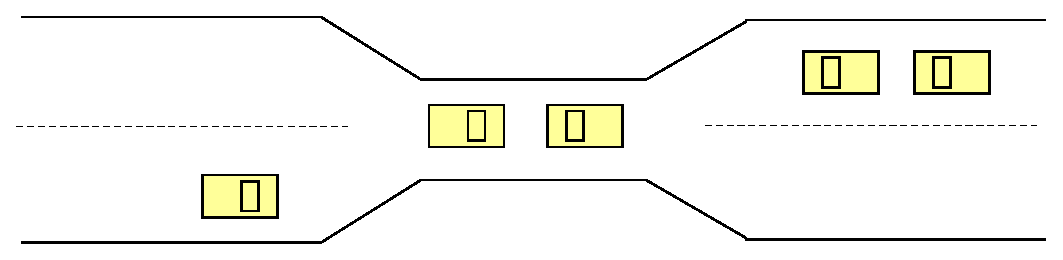
\includegraphics[width=100mm]{figs/bridge}}
% 
% \bigskip
% 
% \itms{
%   \item Real issue is \emph{resources} \& how required
%   \item E.g., bridge only allows traffic in one direction
%   \ittms{
%     \item Each section of a bridge can be viewed as a resource.
%     \item If a deadlock occurs, it can be resolved if one car backs up (preempt resources and rollback).
%     \item Several cars may have to be backed up if a deadlock occurs.
%     \item Starvation is possible.
%   }
% }
% \end{slide}

\begin{slide}{Deadlock conditions}
\itms{
\item[1.] Limited access (mutual exclusion):
\ittms{
\item Resource can only be shared with finite users
}
\item[2.] No preemption: 
\ittms{
\item Once resource granted, cannot be taken away
}
\item[3.] Multiple independent requests (hold and wait):
\ittms{
\item Don't ask all at once\\
  (wait for next resource while holding current one)
}
\item[4.] Circularity in graph of requests
\gap
\item All of 1--4 necessary for deadlock to occur
\item Two approaches to dealing with deadlock: 
\ittms{
\item Pro-active: prevention 
\item Reactive: detection + corrective action 
}
}
\end{slide}

\begin{slide}{Prevent by eliminating one condition}
%\vspace*{-.1in}
\itms{
\item[1.] Limited access (mutual exclusion):
\ittms{
  \item Buy more resources, split into pieces, or virtualize to make
    "infinite" copies 
  \item Threads: threads have copy of registers = no lock
}
\item[2.] No preemption: 
\ittms{
\item Physical memory: virtualized with VM, can take physical page away and give to another process!
}
\item[3.] Multiple independent requests (hold and wait):
\ittms{
\item Wait on all resources at once (must know in advance)
}
\item[4.] \Red{Circularity in graph of requests}
\ittms{
\item Single lock for entire system: (problems?)
\item Partial ordering of resources (next)
}
}
\end{slide}

% \begin{slide}{Resource-allocation graph}
% \itms{
%   \item View system as graph
%   \ittms{
%     \item Processes and Resources are nodes
%     \item Resource Requests and Assignments are edges
%   }
%   \item Process: \lower.5ex\hbox{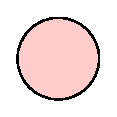
\includegraphics[height=3ex]{figs/ra-proc}}
%   \item Resource w.\ 4 instances: 
%   \lower.5ex\hbox{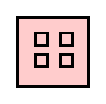
\includegraphics[height=3ex]{figs/ra-resource}}
%   \item $P_i$ requesting $R_j$: 
%     \lower3ex\hbox{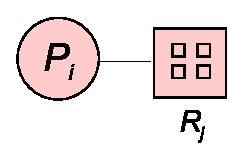
\includegraphics[height=6ex]{figs/ra-req}}
%   \item $P_i$ holding instance of $R_j$:
% \lower3ex\hbox{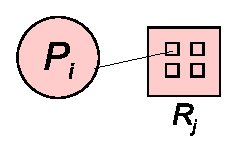
\includegraphics[height=6ex]{figs/ra-hold}}
% }
% \end{slide}
% 
% \begin{slide}{Example resource allocation graph}
% \centerline{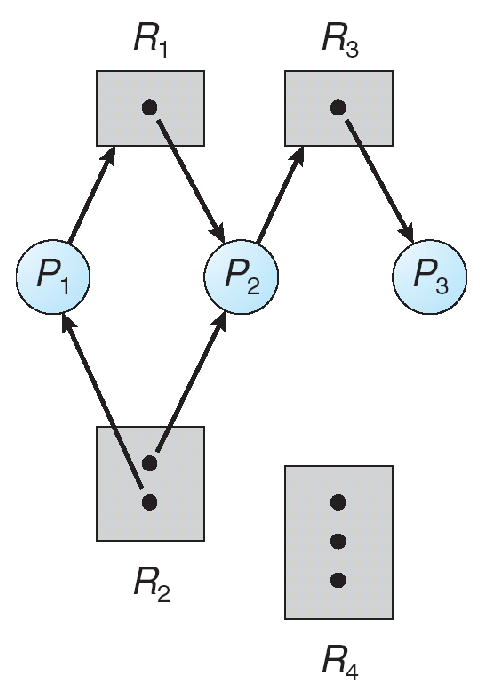
\includegraphics[height=3in]{figs/example-graph}}
% \end{slide}
% 
% \begin{slide}{Graph with deadlock}
% \centerline{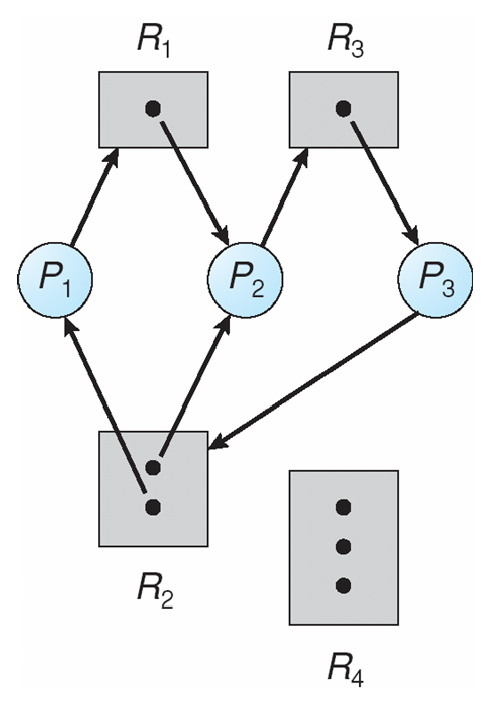
\includegraphics[height=3in]{figs/deadlock-graph}}
% \end{slide}
% 
% \begin{slide}{Is this deadlock?}
% \centerline{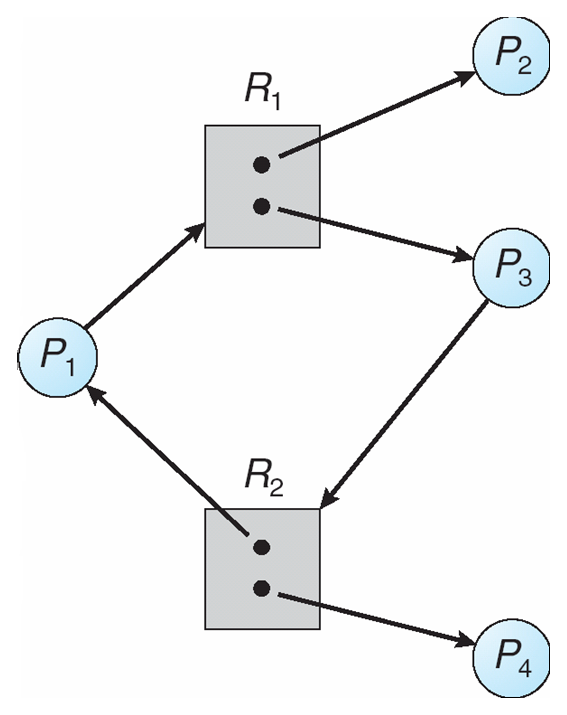
\includegraphics[height=2.7in]{figs/cycle-graph}}
% \end{slide}

\begin{slide}{Cycles and deadlock}
\itms{
  \item View system as graph
  \ittms{
    \item Processes and Resources are nodes
    \item Resource Requests and Assignments are edges
  }
  \gap
  \item If graph has no cycles $\rightarrow$ no deadlock
  \item If graph contains a cycle
  \ittms{
    \item Definitely deadlock if only one instance per resource
    \item Otherwise, maybe deadlock, maybe not
  }
  \gap
  \item Prevent deadlock with partial order on resources
  \ittms{
    \item E.g., always acquire mutex $m_1$ before $m_2$
    \item Statically assert lock ordering (e.g., VMware ESX)
    \item Dynamically find potential deadlocks
	\href{https://www.freebsd.org/cgi/man.cgi?witness(4)}{[Witness]}
  }
}
\end{slide}

% \begin{slide}{Prevention}
% \centerline{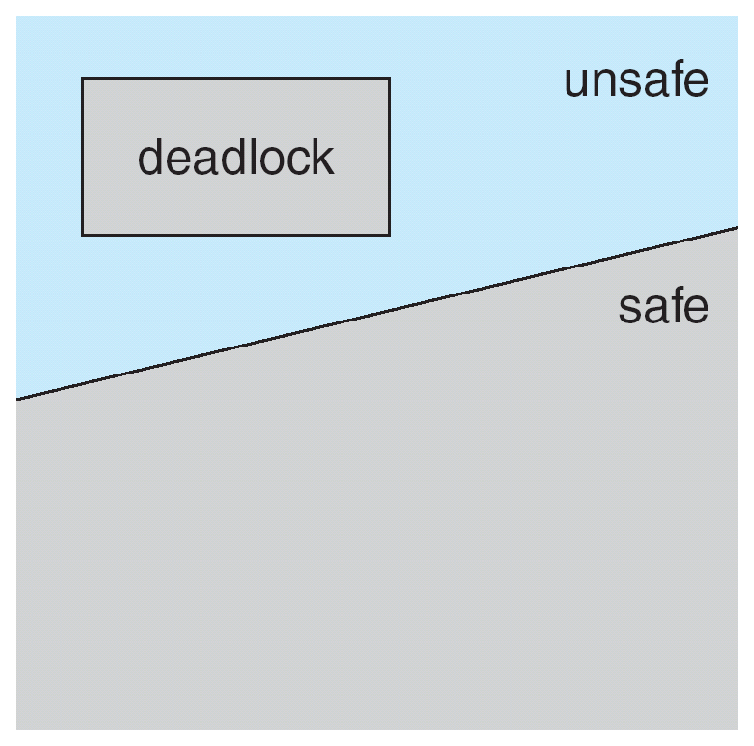
\includegraphics[height=64mm]{figs/safe}}
% \itms{
%   \item Determine safe states based on \emph{possible} resource
% 	    allocation
%   \item Conservatively prohibits non-deadlocked states
% }
% \end{slide}
% 
% \begin{slide}{Claim edges}
% \centerline{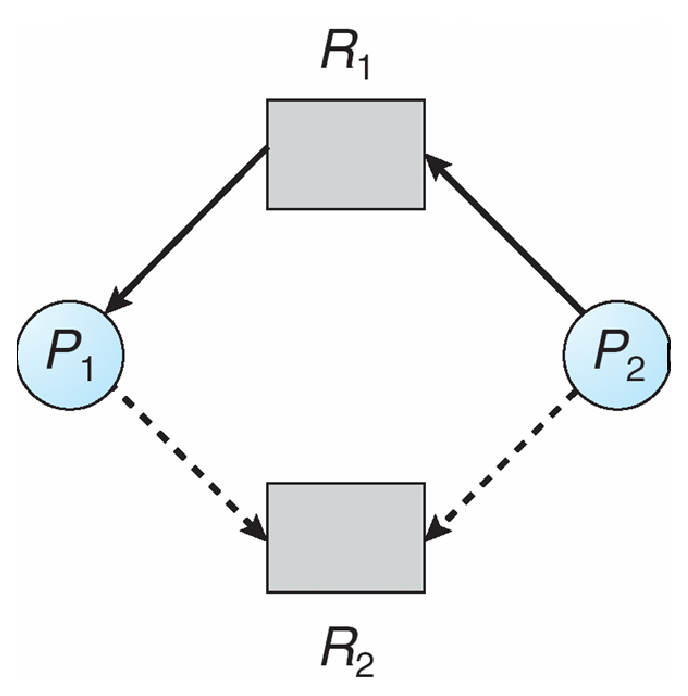
\includegraphics[height=2in]{figs/dotted}}
% \itms{
%   \item Dotted line is \emph{claim edge}
%   \ittms{
%     \item Signifies process \emph{may} request resource
%     \item[]
%   }
% }
% \end{slide}
% 
% \begin{slide}{Example: unsafe state}
% \centerline{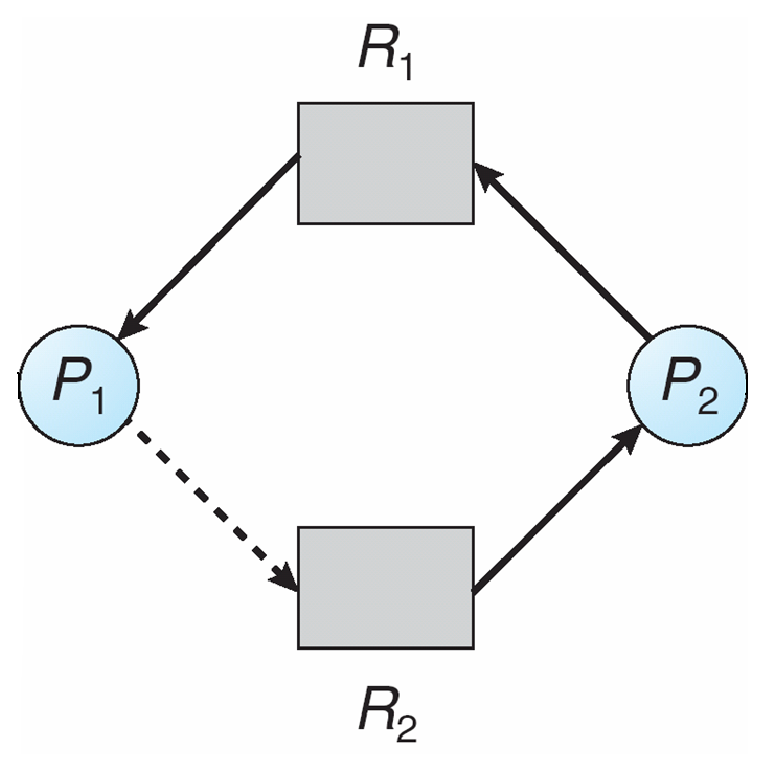
\includegraphics[height=2in]{figs/unsafe}}
% \itms{
%   \item Note cycle in graph
%   \ittms{
%     \item $P_1$ might request $R_2$ before relinquishing $R_1$
%     \item Would cause deadlock
%   }
% }
% \end{slide}
% 
% 
% \begin{slide}{Detecting deadlock}
% \itms{
%   \item Static approaches (hard)
%   \item Program grinds to a halt
%   \item Threads package can keep track of locks held:
% }
% \centerline{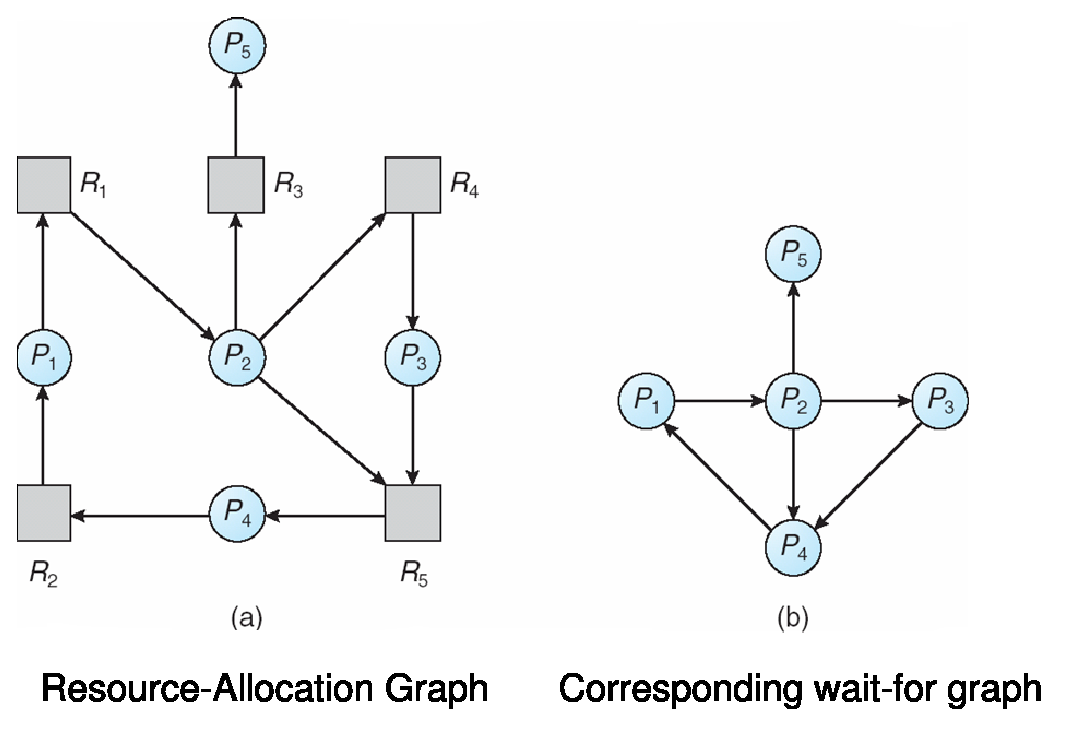
\includegraphics[height=60mm]{figs/detect}}
% \end{slide}

%  \begin{slide}{Fixing \& debugging deadlocks}
%  \itms{
%      \item Reboot system (windows approach)
%      \item Examine hung process with debugger
%      \item Threads package can deduce partial order
%    \ittms{
%      \item For each lock acquired, order with other locks held
%      \item If cycle occurs, abort with error
%      \item Detects \emph{potential} deadlocks even if they do not occur
%    }
%    \item Or use \Red{\emph{transactions}}\ldots
%    \ittms{
%      \item Another paradigm for handling concurrency
%      \item Often provided by databases, but some OSes use them
%      \item \emph{Vino} OS used transactions to abort after failures
%        \href{http://www.eecs.harvard.edu/syrah/vino//osdi-96/paper.html}{[Seltzer]}
%      %\item OS support for transactional memory now hot research topic
%    }
%  %  \item Or with transactions, can just tolerate
%  %  \ittms{
%  %    \item Just abort a transaction when deadlock detected
%  %    \item Safe, though inefficient if it happens often
%  %  }
%  }
%  \end{slide}

% \begin{slide}{Transactions}
% %\vspace*{-.2in}
% \itms{
%   \item A \emph{transaction} $T$ is a collection of actions with
%   \ittms{
%     \item \emph{\Red{A}tomicity} -- all or none of actions happen
%     \item \emph{\Red{C}onsistency} -- $T$ leaves data in valid state
%     \item \emph{\Red{I}solation} -- $T$'s actions all appear to happen
%     before or after every other transaction $T'$
%     \item \emph{\Red{D}urability*} -- $T$'s effects will survive reboots
%     \item Often hear mnemonic \emph{\Red{ACID}} to refer to above
%   }
%   \item Transactions typically executed concurrently
%   \ittms{
%     \item But \emph{isolation} means must \emph{appear} not to
%     \item Must roll-back transactions that use others' state
%     \item Means you have to record all changes to undo them
%   }
%   \item When deadlock detected just abort a transaction
%   \ittms{
%     \item Breaks the dependency cycle
%   }
% }
% \end{slide}
% 
% \begin{frame}
% \frametitle{Transactional memory}
% \begin{itemize}
%   \item Some modern processors support \emph{transactional memory}
%   \item Transactional Synchronization Extensions (TSX)
%       \href{http://www.intel.com/content/dam/www/public/us/en/documents/manuals/64-ia-32-architectures-software-developer-vol-1-manual.pdf\#page=341}{[intel1\S15]}
%   \begin{itemize}
%     \item \texttt{xbegin abort\_handler} -- begins a transaction
%     \item \texttt{xend} -- commit a transaction
%     \item \texttt{xabort \$code} -- abort transaction with 8-bit code
%     \item Note: nested transactions okay (also \texttt{xtest} tests if
%       in transaction)
%   \end{itemize}
%   \item During transaction, processor tracks accessed memory
%   \begin{itemize}
%     \item Keeps read-set and write-set of cache lines
%     \item Nothing gets written back to memory during transaction
%     \item On \texttt{xend} or earlier, transaction aborts if any
%       conflicts
%     \item Otherwise, all dirty cache lines are written back atomically
%   \end{itemize}
% \end{itemize}
% \end{frame}
% 
% \begin{frame}
% \frametitle{Using transactional memory}
% \begin{itemize}
%   \item Use to get ``free'' fine-grained locking on a hash table
%   \begin{itemize}
%     \item E.g., concurrent inserts that don't touch same buckets are okay
%     \item Hardware will detect there was no conflict
%   \end{itemize}
%   \item Use to poll for one of many asynchronous events
%   \begin{itemize}
%     \item Start transaction
%     \item Fill cache with values to which you want to see changes
%     \item Loop until a write causes your transaction to abort
%   \end{itemize}
%   \item Note:  Transactions are never guaranteed to commit
%   \begin{itemize}
%     \item Might overflow cache, get false sharing, see weird processor
%       issue
%     \item Means abort path must always be able to perform transaction
%       \\ (e.g., you do need a lock on your hash table)
%   \end{itemize}
% \end{itemize}
% \end{frame}
% 
% \begin{frame}
% \frametitle{Hardware lock elision (HLE)}
% \begin{itemize}
%   \item Idea: have spinlocks that rarely need to spin
%   \begin{itemize}
%     \item Begin a transaction when you acquire lock
%     \item Other CPUs won't see lock acquired, can also enter critical
%       section
%     \item Okay not to have mutual exclusion when no memory conflicts!
%     \item On conflict, abort and restart without transaction, thereby
%       visibly acquiring lock (and aborting other concurrent
%       transactions)
%   \end{itemize}
%   \item Intel support:
%   \begin{itemize}
%     \item Use \texttt{xacquire} prefix before \texttt{xchgl}
%       (used for test and set)
%     \item Use \texttt{xrelease} prefix before \texttt{movl} that releases
%       lock
%     \item Prefixes chosen to be noops on older CPUs (binary
%       compatibility)
%   \end{itemize}
%   \item Hash table example:
%   \begin{itemize}
%     \item Use \texttt{xacquire xchgl} in table-wide test-and-set spinlock
%     \item Works correctly on older CPUs (with coarse-grained lock)
%     \item Allows safe concurrent accesses on newer CPUs!
%   \end{itemize}
% \end{itemize}
% \end{frame}

%% \begin{slide}{Detecting data races}
%% \itms{
%%   \item Static methods (hard)
%%   \item Debugging painful---race might occur rarely
%%   \item Instrumentation---modify program to trap memory accesses
%%   \item Lockset algorithm (eraser
%%     \href{http://www.cs.ucsd.edu/~savage/papers/Tocs97.pdf}{[Savage]}) particularly effective:
%%   \ittms{
%%     \item For each global memory location, keep a ``lockset''
%%     \item On each access, remove any locks not currently held
%%     \item If lockset becomes empty, abort:  No mutex protects data
%%     \item Catches potential races even if they don't occur
%%   }
%% }
%% \end{slide}

%  \section{Scalable Interface Design}
%  
%  \begin{slide}{Scalable Interfaces}
%  \itms{
%    \item Not all interfaces can scale
%    \item How to tell which can and which can't?
%    \item Scalable Commutativity Rule: \emph{``Whenever interface operations 
%    commute, they can be implemented in a way that scales''} 
%    \href{http://web.mit.edu/amdragon/www/pubs/commutativity-sosp13.pdf}{[Clements]} 
%    }
%  \end{slide}
%  
%  \begin{slide}{Is Fork(), Exec() Broadly Commutative?}
%  \texttt{Fork() -> ret; if (!ret) exec("bash");}
%  \end{slide}
%  
%  \begin{slide}{Is Fork(), Exec() Broadly Commutative?}
%  \texttt{Fork() -> ret; if (!ret) exec("bash");}
%  \itms{
%    \item No, \texttt{fork()} doesn't commute with memory writes, many file descriptor operations, and all address space operations
%    \item \texttt{Exec()} often follows \texttt{fork()} and undoes most of \texttt{fork()}'s sub operations
%    \item \texttt{Posix\_spawn()}, which combines \texttt{fork()} and \texttt{exec()} into a single operation, is broadly commutative
%  }
%  \end{slide}
%  
%  \begin{slide}{Is Open() Broadly Commutative?}
%  \texttt{Open("foo", flags) -> fd1, Open("bar", flags) -> fd2}
%  \end{slide}
%  
%  \begin{slide}{Is Open() Broadly Commutative?}
%  \texttt{Open("foo", flags) -> fd1, Open("bar", flags) -> fd2}
%  \itms{
%    \item Actually \texttt{open()} does not broadly commute!
%    \item Does not commute with any system call (including itself) that creates a file descriptor
%    \item Why? POSIX requires new descriptors to be assigned the lowest available integer
%    \item If we fixed this, \texttt{open()} would commute, as long as it is not creating a file in the same directory as another operation
%  }
%  \end{slide}

\section{OS Implementation}

\begin{slide}{Wait Channels}
\itms{
  \item OS locks (except spinlocks) use wait channels to manage sleeping 
      threads
  \item \code{void wchan_sleep(struct wchan *wc);}
  \ittms{
    \item Blocks calling thread on wait channnel \code{wc}
    \item Causes a context switch (e.g., \code{thread_yield})
  }
  \item \code{void wchan_wakeall(struct wchan *wc);}
  \ittms{
    \item Unblocks all threads sleeping on the wait channel
  }
  \item \code{void wchan_wakeone(struct wchan *wc);}
  \ittms{
    \item Unblocks one threads sleeping on the wait channel
  }
  \item \code{void wchan_lock(struct wchan *wc);}
  \ittms{
    \item Lock wait channel operations
    \item Prevents a race between sleep and wakeone
  }
}
\end{slide}

\begin{slide}{OS/161 Semaphores}
\vspace{-1em}
\begin{smallccode}
P(struct semaphore *sem) {
  spinlock_acquire(&sem->sem_lock);
  while (sem->sem count == 0) {
    /* Locking the wchan prevents a race on sleep */
    wchan_lock(sem->sem wchan);
    /* Release spinlock before sleeping */
    spinlock_release(&sem->sem_lock);
    /* Wait channel protected by it's own lock */
    wchan_sleep(sem->sem wchan);
    /* Recheck condition, no locks held */
    spinlock_acquire(&sem->sem_lock);
  }
  sem->sem count--;
  spinlock release(&sem->sem lock);
}

V(struct semaphore *sem) {
  spinlock_acquire(&sem->sem_lock);
  sem->count++;
  wchan_wakeone(sem->sem wchan);
  spinlock_release(&sem->sem_lock);
}
\end{smallccode}
\end{slide}

\end{document}

